\documentclass{article}

\usepackage{graphicx}

\title{Stability And Evolution Of Conway's Game Of Life}
\author{Leo BECHET  \\
UFR Sciences et Techniques, Besancon, FRANCE \\
leo.bechet@edu.univ-fcomte.fr
	}

\date{\today}
% Hint: \title{what ever}, \author{who care} and \date{when ever} could stand 
% before or after the \begin{document} command 
% BUT the \maketitle command MUST come AFTER the \begin{document} command! 
\begin{document}

\maketitle


\begin{abstract}
Short introduction to subject of the paper \ldots 
\end{abstract}

\section{Introduction}
Conway's Game of Life, conceived by mathematician John Conway in 1970, 
is a cellular automaton operating on a grid of cells. Governed by four 
simple rules, each cell's status is determined by its neighboring cells, 
leading to a rich tapestry of patterns ranging from static formations to 
dynamic entities. Beyond its recreational appeal, the Game of Life finds 
application in scientific domains such as computer science, mathematics, 
and biology. Its enduring significance lies in its ability to stimulate 
inquiry into emergent complexity in various systems. In this article we 
will explore the evolution of the automaton for different starting
conditions.





\section{Experiment context}
The focus lies on exploring the dynamics 
of Conway's Game of Life cellular automaton within a computationally 
feasible framework. The study employs a 500 by 500 grid with wrapping 
around the edges to effectively simulate an infinite grid, thus 
accommodating the inherent spatial constraints of computational 
resources. While acknowledging the potential introduction of periodic 
errors due to wrapping, the experiment adopts the perspective that in 
an infinite grid, such errors would manifest as an infinite grid can be considered as a repetition 
of an infinitely large grid. This approach allows us to 
investigate emergent phenomena and general properties of the Game of 
Life, leveraging the convenience of a finite grid while approximating 
the behavior of an infinite system. 


\section{Initial analysis}
The initial analysis phase of the experiment involves generating random 
grids with varying filling percentages, ranging from 0\% to 100\% filled, 
with each percentage representing a sweep across the spectrum of possible 
initial conditions. For each filling percentage, the simulation is run for 
1000 cycles, allowing the grid to evolve according to the rules of Conway's 
Game of Life cellular automaton. This process is repeated 10 times for 
each percentage to account for stochastic variability in the initial conditions. 
To quantify the equilibrium filling of the grid at each percentage, 20 evenly 
distributed points are selected across the simulation timeline. The final 
filled percentage is computed as the average of the last points of each of the 
10 simulations conducted for that particular percentage. These average values 
are then plotted to generate a graph illustrating the relationship between the 
initial filling percentage and the corresponding equilibrium filling state. The resulting 
graph is given in 

\begin{figure}[htbp]
    \centering
    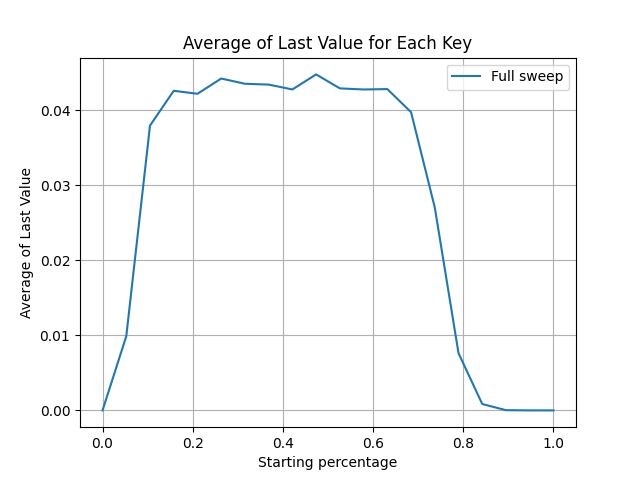
\includegraphics[width=0.8\textwidth]{res/full_start_finish.png}
    \caption{Final filling percentage for a sweep of 20 points accross 0\% to 100\% starting filling.}
    \label{fig:full}
\end{figure}

After conducting the initial simulations, it was observed in Fig \ref*{fig:full} that the final percentage 
of filled cells exhibits a non-linear trend with respect to the initial filling percentage. 
Initially, from 0\% to 10\% starting filling, the final percentage rises. 
Subsequently, between 10\% and 70\% initial filling, the final percentage stabilizes 
at around 4.5\%. Beyond 70\% initial filling, the final percentage begins to decline 
once again. This pattern suggests that the dynamics of Conway's Game of Life cellular 
automaton exhibit distinct behaviors at different ranges of initial filling percentages. 
The initial rise in final filling percentage may reflect the propagation and expansion of 
patterns from initially sparse configurations, while the subsequent stabilization could 
indicate a balance between birth and death rates of cells within moderately filled grids. 
The observed decline in final percentage at higher initial fillings may be attributed to 
increased competition and limited space for the growth and sustainability of patterns, 
leading to more frequent cell deaths. These findings highlight the intricate interplay 
between initial conditions and emergent behaviors in cellular automata systems. Further 
analysis and modeling efforts are warranted to fully elucidate the underlying mechanisms 
driving these observed phenomena. Moreover the plateau observed at 4.5\% in the final 
percentage of filled cells suggests the presence of a stable equilibrium state within 
Conway's Game of Life, indicating a critical threshold where the interplay between cell 
birth and death rates leads to sustained patterns and structures within the system.

\section{Investigating the first rise}
Due to the resolution of our graph, we do not have much precision on the first rise. Thus
we run 2 other simulations in order to increase the precision on that specific part.


\begin{figure}[htbp]
    \centering
    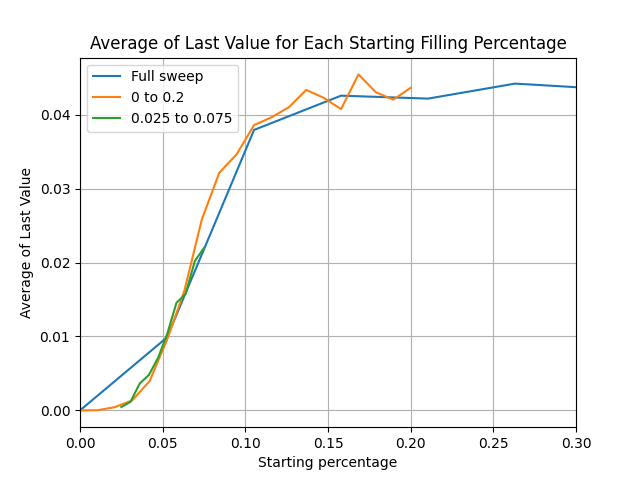
\includegraphics[width=0.8\textwidth]{res/sweep_zoom.png}
    \caption{Increased resolution sweep on the first rise.}
    \label{fig:sweep_zoom}
\end{figure}


In Fig \ref*{fig:sweep_zoom}, the medium curve in orange gives us some insight on the evolution
at low fillings. The highest resolution curve in green does not show much deviation
from the previous curve. Though we would have expected a steeper curve, it appears to slowly go up
in a quadratic fascion. We however speculate\footnote[1]{Due to the complexity of the computations, and a loss of access
to the CompuPhys server, we weren't able to investigate this supposition.} that for an infinite amount of cycle, the final sweep will be 
close to a gate function. 



\section{Evolution in time}
We consider by evolution in time, the evolution of the automaton in relation to each step.
In Fig \ref*{fig:full_evolution} we plot the previous data by averaging each the sets of 
10 runs for each percentages.

\begin{figure}[htbp]
    \centering
    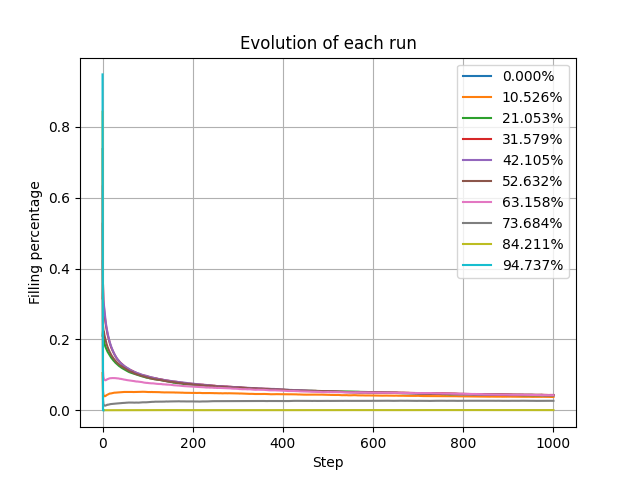
\includegraphics[width=0.8\textwidth]{res/Full_evolution.png}
    \caption{Evolution of the system for different starting fills.}
    \label{fig:full_evolution}
\end{figure}

One aspect of the graph that can be spotted is that both 0\% and 100\% curves go 
straight to a 0\% population. The simulation has checks to stop runs
once if the population reaches 0\%, thus we don't have any steps for those.
The current graph only plots half of the test fills as to not overload the graph.

Second aspect, is that we can see a heavy decrease down under 4.5\% for each percentages.
However, zooming in on the lower part of the graph, it is obvious that the evolution 
does not always follow a exponential decrease. As shown on Fig \ref*{fig:evolution_zoom}, some rise up.
This behavior is consistent for curves where the starting percentage isn't in the plateau identified
of Fig \ref*{fig:full}.

Comparing with Fig \ref*{fig:full}, curves categorized inside the plateau appear to do follow the
exponential decrease. However for the 63\% curve, it appears that it starts with an
important fall before rising up again. We do not know if that value is indeed inside
of the plateau or slitghtly off.
\begin{figure}[htbp]
    \centering
    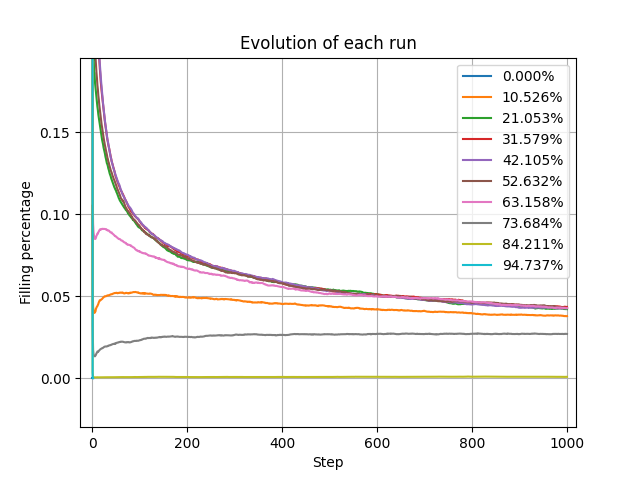
\includegraphics[width=0.8\textwidth]{res/evolution_zoom.png}
    \caption{Evolution of the system for different starting fills zoomed on the lower part.}
    \label{fig:evolution_zoom}
\end{figure}

\section{Fitting to an exponential decrease}
In order to obtain a precise value for the plateau, we propose to fit one of the central
curve to an exponential decay described in Eq. \ref*{eq:exp_decay}.

\begin{equation}
    f(x) = e^{-ax + b} + c
    \label{eq:exp_decay}
\end{equation}

The following fit resulted in values of $a=0.00364699$, $b=-2.62888693$,
$c=0.04145781$. The comparison between the points and the fit is displayed in 
Fig \ref*{fig:decay_fit}. Fitting the whole data was not possible due to the first points.
We believe that though the exponential decay looks to be a correct fit, it
does not correspond to the right function. Fits using an inverse function were
inconclusive. From the value of C, we expect that the plateau is around 4.1\%
of population. It is however necessary to state that we have no proof that it is
flat, and it might aswell be bumped. The bump theory actually makes sense by allowing
descrepancies in the final value for limited number of iterations, while still leaving the 
possibility of all percentage inside the plateau to converge to the same value for an infinite number
of cycle. 

\begin{figure}[htbp]
    \centering
    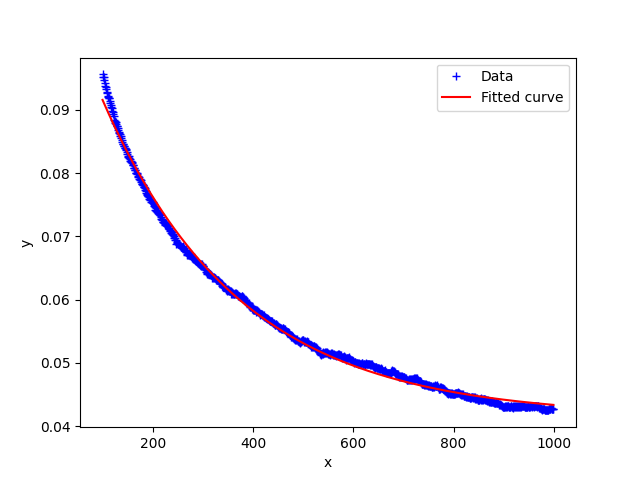
\includegraphics[width=0.8\textwidth]{res/fit.png}
    \caption{Fitting of the 42\% curve to Eq. \ref*{eq:exp_decay}}
    \label{fig:decay_fit}
\end{figure}

% \paragraph{Outline}
% First we start with a little example of the article class, which is an 
% important documentclass. But there would be other documentclasses like 
% book \ref{book}, report \ref{report} and letter \ref{letter} which are 
% described in Section \ref{documentclasses}. Finally, Section 
% \ref{conclusions} gives the conclusions.



% \section{Documentclasses} \label{documentclasses}

% \begin{itemize}
% \item article
% \item book 
% \item report 
% \item letter 
% \end{itemize}


% \begin{enumerate}
% \item article
% \item book 
% \item report 
% \item letter 
% \end{enumerate}

% \begin{description}
% \item[article\label{article}]{Article is \ldots}
% \item[book\label{book}]{The book class \ldots}
% \item[report\label{report}]{Report gives you \ldots}
% \item[letter\label{letter}]{If you want to write a letter.}
% \end{description}


% \section{Conclusions}\label{conclusions}
% There is no longer \LaTeX{} example which was written by \cite{doe}.


% \begin{thebibliography}{9}
% \bibitem[Doe]{doe} \emph{First and last \LaTeX{} example.},
% John Doe 50 B.C. 
% \end{thebibliography}

\end{document}